\documentclass{article}
\usepackage{geometry}  
\usepackage{amsmath}  
\usepackage{graphicx} 
\usepackage{svg}
\usepackage[T1]{fontenc}
\usepackage{float}
\usepackage{array}

\title{Programowanie układów rekonfigurowalnych \\ Laboratorium 4-5 \\} % Report title

\author{Anna \textsc{Dzieżyk}, indeks: 318506}% Author name(s), add additional authors like: '\& James \textsc{Smith}'

\date{20.01.2025} % Date of the report
\begin{document}

\maketitle % Insert the title, author and date using the information specified above

\begin{center}
	\begin{tabular}{l r}
		Data wykonania ćwiczenia: & 16 stycznia 2025 \\ % Date the experiment was performed
		Prowadzący: & dr hab. inż. Andrzej \textsc{Wojeński} % Instructor/supervisor
	\end{tabular}
\end{center}

\section{CEL}
Celem projektu było stworzenie systemu modułowego do zarządzania światełkami LED o dwóch przydzielonych
przez prowadzącego funkcjach: \\
Wariant 2: Diody świecące naprzemiennie (co druga)\\
Wariant 7: Diody włączające się kolejno, aż do 8 włączonych, a następnie kolejno wyłączające się.\\
Koniecznością w zaimplementowaniu zarządzania diodami jest:\\
- możliwość zmiany wariantu świecenia LEDów na inny przez wciśnięcie przycisku, \\
- możliwość wyłączenia świecenia diód przyciskiem \\
- możliwiść przyspieszenia pracy diód przyciskiem \\
Wymogiem przy użyciu przycisków jest implementacja modułu tzw. Deboucera, który ma przeciwdziałać drganiu styków. Ponadto samo 
zarządzanie prędkością zmiany "mrugania" diod dla jednego wariantu świecenia też musiało być zaimplementowane jako osobny moduł tzw.: Prescaler.
Cel projektu został zrealizowany - w dalszych punktach znajduje się struktura systemu jako schemat blokowy wygenerowany przez Vivado oraz jego omówienie.
\section{WYNIK SYNTEZY}
\subsection{Schemat blokowy}
\begin{figure} [H]
	\begin{center}
			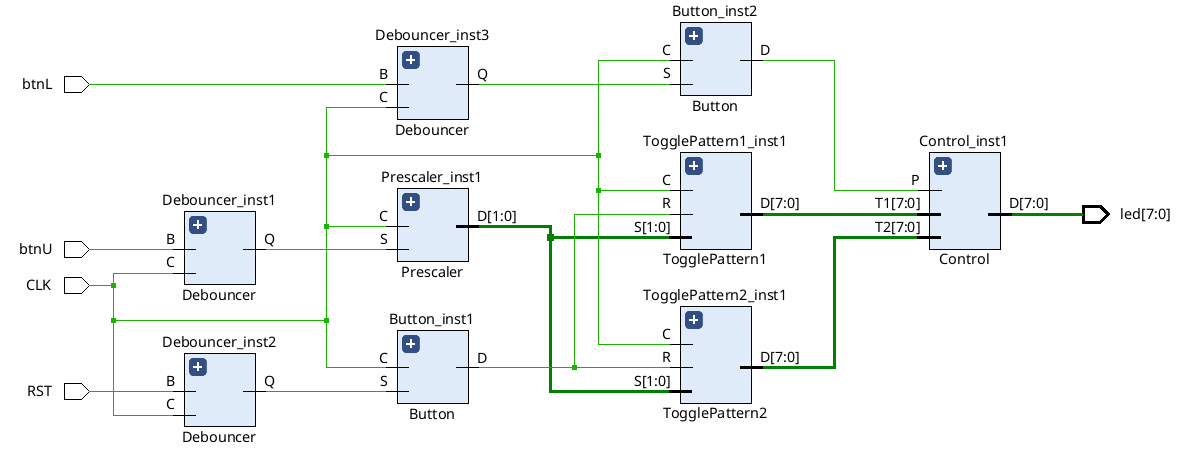
\includegraphics[width = \textwidth]{schematBlokowy.png}
			\caption{Schemat blokowy zaprojektowanego systemu}
\end{center}
\end{figure}
\subsection{Zużycie zasobów}
\begin{figure} [H]
	\begin{center}
			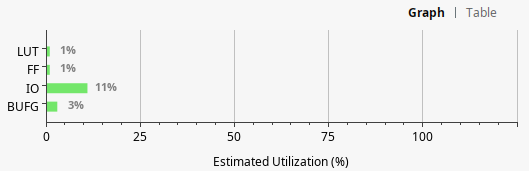
\includegraphics[width = \textwidth]{zasobyPoSynth.png}
			\caption{Zużycie zasobów po syntezie}
\end{center}
\end{figure}
\begin{figure} [H]
	\begin{center}
			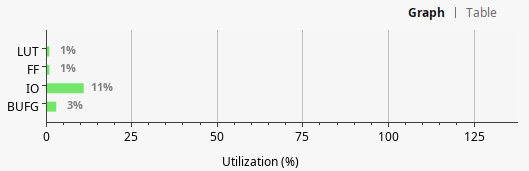
\includegraphics[width = \textwidth]{zasobyPoImpl.png}
			\caption{Zużycie zasobów po implemetacji}
\end{center}
\end{figure}
\section{OPRACOWANY KOD POSZCZEGÓLNYCH MODUŁÓW}
\subsection{Debouncer}
\begin{table}[h]
    \centering
    \begin{tabular}{|c|c|c|}
        \hline
        Nazwa sygnału & Typ sygnału & Opis \\
        \hline
        C  & wejściowy (1-bit)    & sygnał zegarowy    \\
        \hline
        B  & wejściowy (1-bit)   & surowy sygnał stanu przycisku    \\
        \hline
        Q  & wyjściowy (1-bit)   & wykrycie wciśnięcia    \\
        \hline
        counter  & wewnętrzny (liczba)    & licznik     \\
        \hline
        Q1  & wewnętrzny (1-bit) & wyjście pierwszego zatrzasku typu D   \\
        \hline
        Q2  & wewnętrzny (1-bit)  & wyjście drugiego zatrzasku typu D\\
        \hline
    \end{tabular}\\
    \caption{Tabelka sygnałów modułu}
    \label{tab:tabela1}
\end{table}
Zasada działania: W przykadku wykrycia stabilnego wciśnięcia, na wyjściu Q pojawia się krótki impuls 0->1->0 świadczący o tym, że 
    przycisk został stabilnie wciśnięty. Implementacja opiera się na zliczaniu do określonej wartości, które odbywa się tak długo, jak stan 
    przycisku jest niezmieniony i jest wysoki. W przypadku doliczenia do tej wartości, zatraskiwany jest stan przycisku najpierw w jednym zatrzasku typu D, a po
    kolejnym zliczeniu do określonej wartości, w drugim. Impuls wyjsicowy to suma zanegowanego wyścia z drugiego zatrzasku i niezmienionego wyjścia pierwszego zatrzsku.
\subsection{Button}
\begin{table}[H]
    \centering
    \begin{tabular}{|c|c|c|}
        \hline
        Nazwa sygnału & Typ sygnału & Opis \\
        \hline
        C  & wejściowy (1-bit)    & sygnał zegarowy    \\
        \hline
        S  & wejściowy (1-bit)   & Sygnał impulsów do zliczania    \\
        \hline
        D  & wyjściowy (1-bit)    & sygnał indukujący wciśnięcie\\
        \hline
        toggle  & wewnętrzny (1-bit)    & sygnał przełączający 1-0\\
        \hline
        prev\_s  & wewnętrzny (1-bit) & poprzedni stan do wykrywania zbocza \\
        \hline
    \end{tabular}\\
    \caption{Tabelka sygnałów modułu}
    \label{tab:tabela2}
\end{table}
Zasada działania: W przypadku wykrycia impulsu, który mówi, że przycisk został wciśnięty, stan na wyjściu modułu jest negowany. Czyli moduł 
implementuje zliczanie do 2 jako licznik jednobitowy. 
\subsection{Prescaler}
\begin{table}[H]
    \centering
    \begin{tabular}{|c|c|c|}
        \hline
        Nazwa sygnału & Typ sygnału & Opis \\
        \hline
        C  & wejściowy (1-bit)    & sygnał zegarowy    \\
        \hline
        S  & wejściowy (1-bit)   & Sygnał impulsów do zliczania    \\
        \hline
        D  & wyjściowy (2-bit)    & sygnał zliczonych impulsów\\
        \hline
        counter  & wewnętrzny (liczba)    & licznik\\
        \hline
        prev\_s  & wewnętrzny (1-bit) & poprzedni stan do wykrywania zbocza \\
        \hline
    \end{tabular}\\
    \caption{Tabelka sygnałów modułu}
    \label{tab:tabela3}
\end{table}
Zasada działania: W przypadku wykrycia wciśnięcia przycisku, czyli gdy na wejście modułu trafia sygnał z Debouncera, do obecnej wartości na wyjściu dodawany jest 1. 
Innymi słowy moduł implementuje licznik 2-bitowy, zliczający do 4 - na wyjściu mogą się pojawić 4 stanu: 00, 01, 10, 11.
\subsection{TogglePattern1}
\begin{table}[H]
    \centering
    \begin{tabular}{|c|c|c|}
        \hline
        Nazwa sygnału & Typ sygnału & Opis \\
        \hline
        C  & wejściowy (1-bit)    & sygnał zegarowy    \\
        \hline
        R  & wejściowy (1-bit)   & sygnał resetu   \\
        \hline
        S  & wejściowy (2-bit)    & sygnał szybkości mrugania\\
        \hline
        D  & wyjściowy (7-bit)    & sygnał wyjściowy\\
        \hline
        T  & wewnętrzny (stała liczba) & stała zakresu zliczania przez T  \\
        \hline
        L  & wewnętrzny (liczba) & sygnał licznika \\
        \hline
        Z  & wewnętrzny (liczba) & sygnał zakresu zliczania \\
        \hline
    \end{tabular}\\
    \caption{Tabelka sygnałów modułu}
    \label{tab:tabela4}
\end{table}
Zasada działania: Stan wyjściowy D zmienia się między wektorami "10101010", a "01010101" co każde zliczenie licznika do liczby, która jest ustalana w 
zależności od zakresu zliczania Z. Zakres zliczania zależy od stanu wyjściowego prescalera. Moduł wystawia same zera na wyjściu, gdy sygnał R - wyboru modułu - jest równy 0. 
\subsection{TogglePattern2}
\begin{table}[H]
    \centering
    \begin{tabular}{|c|c|c|}
        \hline
        Nazwa sygnału & Typ sygnału & Opis \\
        \hline
        C  & wejściowy (1-bit)    & sygnał zegarowy    \\
        \hline
        R  & wejściowy (1-bit)   & sygnał resetu   \\
        \hline
        S  & wejściowy (2-bit)    & sygnał szybkości mrugania\\
        \hline
        D  & wyjściowy (7-bit)    & sygnał wyjściowy\\
        \hline
        T  & wewnętrzny (stała liczba) & stała zakresu zliczania przez T  \\
        \hline
        L  & wewnętrzny (liczba) & sygnał licznika \\
        \hline
        Z  & wewnętrzny (liczba) & sygnał zakresu zliczania \\
        \hline
        D\_internal  & wewnętrzny (7-bit) & pomocniczy sygnał wyjścia  \\
        \hline
        direction  & wewnętrzny (1-bit) & kiedunek zmiany \\
        \hline
    \end{tabular}\\
    \caption{Tabelka sygnałów modułu}
    \label{tab:tabela5}
\end{table}
Zasada działania: Co każde zliczenie licznika do zadanego zakresu - zapalana jest kolejna dioda: startujemy z punktu "00000000"->zliczenie do zakresu->"00000001"->... itd.
W przypadku wektora "11111111" - diody gasną w podobny sposób: "11111111" -> "01111111"->...itd. Kierunek zmiany jest determinowany przez sygnał direction i ustawiany za każdym razem na przeciwny, kiedy
wektor D\_internal jest w "skrajnym" stanie (same zera lub same jedynki). Szybkość zmian jest ustalana przez sygnał S - w zależności od jego
wartości mamy zmieniony zakres zliczania Z. Jeżeli sygnał wyboru wariantu mrugania R jest w stanie wysokim (1), moduł wystawia zawsze wektor zer na wyjście.
\subsection{Control}
\begin{table}[H]
    \centering
    \begin{tabular}{|c|c|c|}
        \hline
        Nazwa sygnału & Typ sygnału & Opis \\
        \hline
        T1  & wejściowy (7-bit)    & sygnał mrugania wariantu 2    \\
        \hline
        T2  & wejściowy (1-bit)   & sygnał mrugania wariantu 7    \\
        \hline
        P  & wyjściowy (1-bit)    & sygnał włączenia/wyłączenia\\
        \hline
        D  & wewnętrzny (7-bit)    & sygnał wyjsciowy\\
        \hline
    \end{tabular}\\
    \caption{Tabelka sygnałów modułu}
    \label{tab:tabela6}
\end{table}
Zasada działania: Wyjście D to suma sygnałów T1 i T2. moduły TogglePattern1 i TogglePattern2 umożliwiają takie rozwiązanie, ponieważ nie działają nigdy w tym samym czasie - 
dba o to sygnał R. W module Contol jest również zaimplenetowane to, czy moduł ma działać - jeżeli sygnał P jest równy 1 to cały system działa - diody się zapalają.
\subsection{Moduł TOP - LED\_management}
Moduł ten jest "sklejeniem" wszystkich modułów opisanych powyżej w jedną, spójną całość. W punkcie 2 znajduje się schemat blokowy tego modułu. Warte odnotowania jest to, że moduł 
Deboucera używany jest 3-krotnie: \\
- w przypadku przycisku implementującego wybór wariantu świecenia, impulsy wyjścia debouncera są zliczane do 2 przez moduł Button (licznik 1-bitowy), a wyjście modułu Button podączone jest do
obydwu modułów wariantu świecenia. \\
- w przypadku włączenia/wyłączenia systemu, impulsy są zliczane w ten sam sposób, co w przypadku przycisku odpoweidzialnego za wybór wariantu - też na wyjscie Debouncera
podłączony jest moduł Button, zliczający wciśnięcia do 2 - następnie sygnał ten jest brany pod uwagę w module Control - on decyduje o tym, czy diody mają świecić. \\
- w przypadku wyboru szybkości świcenia, wyjście Debouncera jest podłączone do Prescalera - modułu liznika 2-bitowego, który na wyjściu wystawia w formie 2-bitowego wektora liczbę stabilnych 
wciśnięć przycisku.

W tym module również jest wykonane rzutowanie sygnałów abstrakcyjnych, opisanych wyżej, jako wejścia modułów "zewnętrznych", na rzeczywiste zasoby sprzętowem+, które musiały się
zgadzać z nazwami instancji zasobów płytki opisanymi w pliku *.xdc. Poniższa tabelka przedstawia te sygnały:
\begin{table}[H]
    \centering
    \begin{tabular}{|c|c|c|}
        \hline
        Nazwa sygnału & Typ sygnału & Opis \\
        \hline
        CLK  & wejściowy (1-bit)    & sygnał zegarowy    \\
        \hline
        RST  & wejściowy (1-bit)   & sygnał wyboru wariantu mrugania    \\
        \hline
        btnU  & wejściowy (1-bit)    & sygnał zmiany prędkości\\
        \hline
        btnL  & wejściowy (1-bit)    & sygnał włącz/wyłącz\\
        \hline
        led  & wyjściowy (7-bit)    & sygnał wyjściowy ledów\\
        \hline
    \end{tabular}\\
    \caption{Tabelka sygnałów modułu}
    \label{tab:tabela7}
\end{table}
\section{PODSUMOWANIE ORAZ WYNIKI}
\subsection{Testbench modułów odpowiedzialnych za obsługę przycisków zmiany szybkości mrugania i wybór wariantu}
Testowane tutaj były moduły połączone wg. nastepujacego schematu blokowego:
\begin{figure} [H]
	\begin{center}
			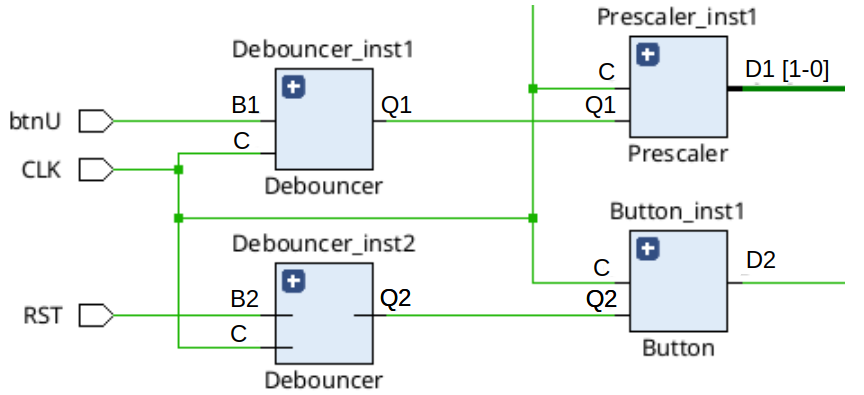
\includegraphics[scale = 0.5]{testbench1.png}
			\caption{Schemat blokowy analizowanego układu w testbenchu}
\end{center}
\end{figure}
Nazwy występujące na schemacie blokowym pokrywają się z nazwami na poniższych przebiegach czasowych.
\begin{figure} [H]
	\begin{center}
			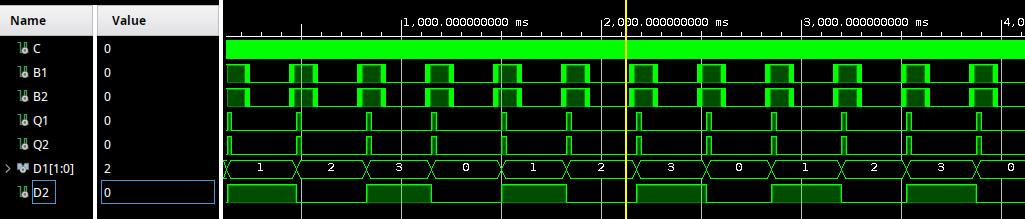
\includegraphics[width = \textwidth]{przebiegi1.png}
			\caption{Przebiegi czasowe analizowanych modułów}
\end{center}
\end{figure}
Wartym zaznaczenia jest, w jaki sposób symulowane było drganie styków - sygnału podawane jako "surowe" sygnały z przycisków symulowane były przez
synchroniczne bardzo szybkie zmiany stanu sygnału trwajace około 12-15 ms, nastepnie podawanie stałego stanu (1 lub 0) i kolejne "zaszumianie" sygnału przy zmianie stanu "stabilnego".

Testbench działa poprawnie, sygnał D1 - jako wyjście licznika 2-bitowego zlicza poprawnie do 4, a sygnał D2, jako wyjście licznika 1-bitowego, poprawnie wystawia stan 0 lub 1 
w zależności od wykrycia wciśnięcia symulowanego przycisku.

\subsection{Testbench całego systemu}
Moduły zostału podłączone wg. następującego schematu blokowego: (proszę zwrócić uwagę na nazwy sygnałów, są korespondujące tym, które 
znajduja się na przebiegach czasowych).

\begin{figure} [H]
	\begin{center}
			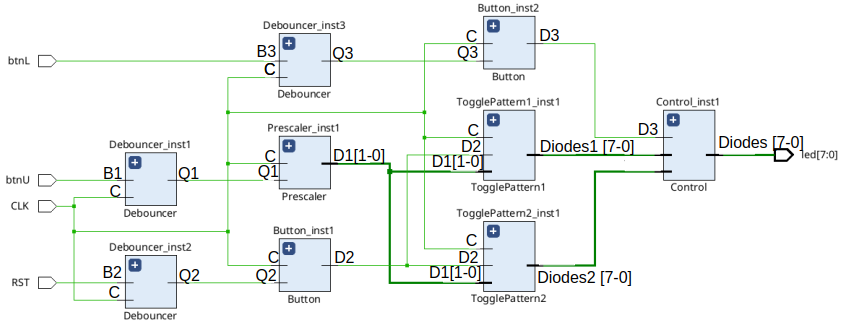
\includegraphics[scale = 0.5]{schemat_blok.png}
			\caption{Schemat blokowy analizowanego układu w testbenchu}
\end{center}
\end{figure}

\begin{figure} [H]
	\begin{center}
			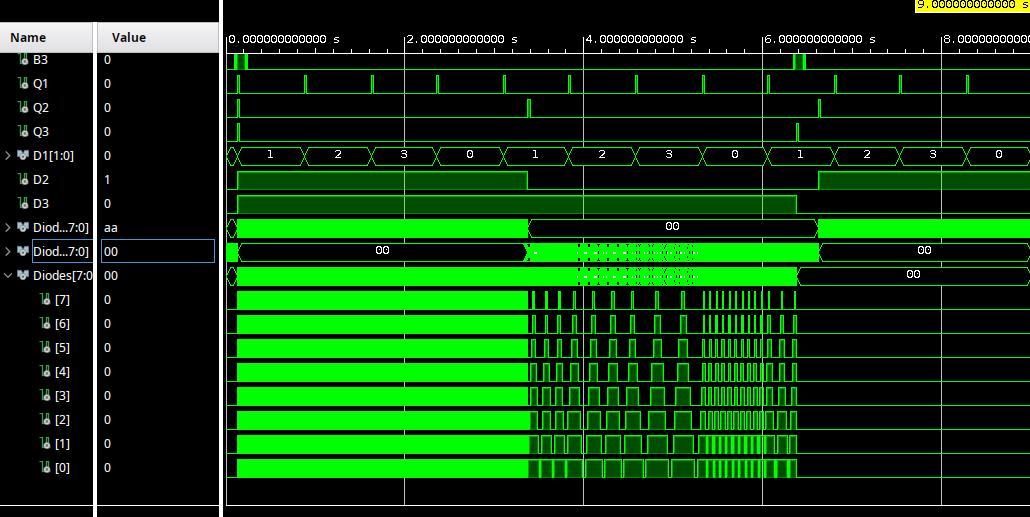
\includegraphics[width = \textwidth]{test2.png}
			\caption{Przebiegi czasowe analizowanych modułów}
\end{center}
\end{figure}
Powyższe przebiegi maja za zadanie pokazać, że analizowane były 3 stany - gdy wybrany ył wariant 2 świecenia diód, gdy wybrany był wariant 7 świecenia diód, oraz gdy układ miał był wyłączony. 
Z tego ogólnego zrzutu przebiegów można stiwerdzić, że moduł Control działa zgodnie z założeniami, a logika sterująca tym, kiedy na wyjściu modułów TogglePattern1 oraz TogglePattern2 pojawia się wektor zer również działa poprawnie.
Dalej sprawdzana będzie poprawność działania zmiany szybkości świecenia diód
\begin{figure} [H]
	\begin{center}
			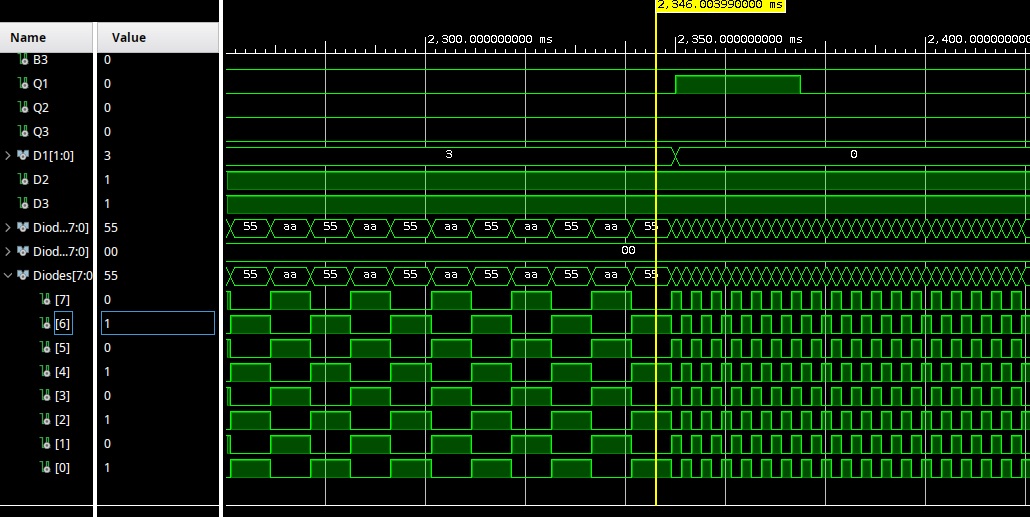
\includegraphics[width = \textwidth]{zmiana1.png}
			\caption{Przykładowa zmiana szybkości świecenia, gdy działa wariant 2}
\end{center}
\end{figure}
\begin{figure} [H]
	\begin{center}
			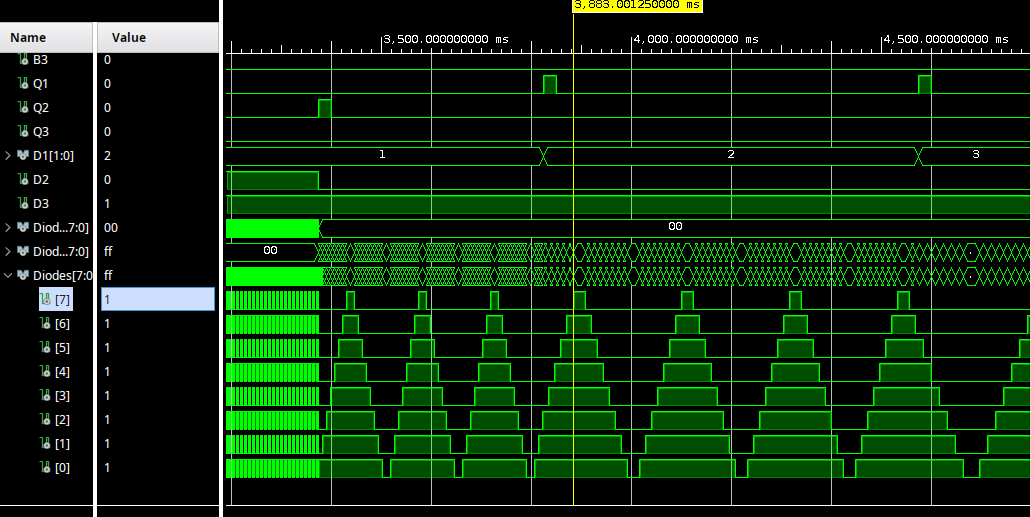
\includegraphics[width = \textwidth]{zmiana2.png}
			\caption{Przykładowa zmiana szybkości świecenia, gdy działa wariant 7}
\end{center}
\end{figure}

Po pierwsze - można uznać, że moduły sterowania diodami działają poprawnie dla poszczególnych prędkości. Zmiany prędkości też są wykonywane poprawnie. Po przetestowaniu na sprzęcie - system również działał oprawnie.
\end{document}